
% Default to the notebook output style

    


% Inherit from the specified cell style.




    
\documentclass[11pt]{article}

    
    
    \usepackage[T1]{fontenc}
    % Nicer default font (+ math font) than Computer Modern for most use cases
    \usepackage{mathpazo}

    % Basic figure setup, for now with no caption control since it's done
    % automatically by Pandoc (which extracts ![](path) syntax from Markdown).
    \usepackage{graphicx}
    % We will generate all images so they have a width \maxwidth. This means
    % that they will get their normal width if they fit onto the page, but
    % are scaled down if they would overflow the margins.
    \makeatletter
    \def\maxwidth{\ifdim\Gin@nat@width>\linewidth\linewidth
    \else\Gin@nat@width\fi}
    \makeatother
    \let\Oldincludegraphics\includegraphics
    % Set max figure width to be 80% of text width, for now hardcoded.
    \renewcommand{\includegraphics}[1]{\Oldincludegraphics[width=.8\maxwidth]{#1}}
    % Ensure that by default, figures have no caption (until we provide a
    % proper Figure object with a Caption API and a way to capture that
    % in the conversion process - todo).
    \usepackage{caption}
    \DeclareCaptionLabelFormat{nolabel}{}
    \captionsetup{labelformat=nolabel}

    \usepackage{adjustbox} % Used to constrain images to a maximum size 
    \usepackage{xcolor} % Allow colors to be defined
    \usepackage{enumerate} % Needed for markdown enumerations to work
    \usepackage{geometry} % Used to adjust the document margins
    \usepackage{amsmath} % Equations
    \usepackage{amssymb} % Equations
    \usepackage{textcomp} % defines textquotesingle
    % Hack from http://tex.stackexchange.com/a/47451/13684:
    \AtBeginDocument{%
        \def\PYZsq{\textquotesingle}% Upright quotes in Pygmentized code
    }
    \usepackage{upquote} % Upright quotes for verbatim code
    \usepackage{eurosym} % defines \euro
    \usepackage[mathletters]{ucs} % Extended unicode (utf-8) support
    \usepackage[utf8x]{inputenc} % Allow utf-8 characters in the tex document
    \usepackage{fancyvrb} % verbatim replacement that allows latex
    \usepackage{grffile} % extends the file name processing of package graphics 
                         % to support a larger range 
    % The hyperref package gives us a pdf with properly built
    % internal navigation ('pdf bookmarks' for the table of contents,
    % internal cross-reference links, web links for URLs, etc.)
    \usepackage{hyperref}
    \usepackage{longtable} % longtable support required by pandoc >1.10
    \usepackage{booktabs}  % table support for pandoc > 1.12.2
    \usepackage[inline]{enumitem} % IRkernel/repr support (it uses the enumerate* environment)
    \usepackage[normalem]{ulem} % ulem is needed to support strikethroughs (\sout)
                                % normalem makes italics be italics, not underlines
    

    
    
    % Colors for the hyperref package
    \definecolor{urlcolor}{rgb}{0,.145,.698}
    \definecolor{linkcolor}{rgb}{.71,0.21,0.01}
    \definecolor{citecolor}{rgb}{.12,.54,.11}

    % ANSI colors
    \definecolor{ansi-black}{HTML}{3E424D}
    \definecolor{ansi-black-intense}{HTML}{282C36}
    \definecolor{ansi-red}{HTML}{E75C58}
    \definecolor{ansi-red-intense}{HTML}{B22B31}
    \definecolor{ansi-green}{HTML}{00A250}
    \definecolor{ansi-green-intense}{HTML}{007427}
    \definecolor{ansi-yellow}{HTML}{DDB62B}
    \definecolor{ansi-yellow-intense}{HTML}{B27D12}
    \definecolor{ansi-blue}{HTML}{208FFB}
    \definecolor{ansi-blue-intense}{HTML}{0065CA}
    \definecolor{ansi-magenta}{HTML}{D160C4}
    \definecolor{ansi-magenta-intense}{HTML}{A03196}
    \definecolor{ansi-cyan}{HTML}{60C6C8}
    \definecolor{ansi-cyan-intense}{HTML}{258F8F}
    \definecolor{ansi-white}{HTML}{C5C1B4}
    \definecolor{ansi-white-intense}{HTML}{A1A6B2}

    % commands and environments needed by pandoc snippets
    % extracted from the output of `pandoc -s`
    \providecommand{\tightlist}{%
      \setlength{\itemsep}{0pt}\setlength{\parskip}{0pt}}
    \DefineVerbatimEnvironment{Highlighting}{Verbatim}{commandchars=\\\{\}}
    % Add ',fontsize=\small' for more characters per line
    \newenvironment{Shaded}{}{}
    \newcommand{\KeywordTok}[1]{\textcolor[rgb]{0.00,0.44,0.13}{\textbf{{#1}}}}
    \newcommand{\DataTypeTok}[1]{\textcolor[rgb]{0.56,0.13,0.00}{{#1}}}
    \newcommand{\DecValTok}[1]{\textcolor[rgb]{0.25,0.63,0.44}{{#1}}}
    \newcommand{\BaseNTok}[1]{\textcolor[rgb]{0.25,0.63,0.44}{{#1}}}
    \newcommand{\FloatTok}[1]{\textcolor[rgb]{0.25,0.63,0.44}{{#1}}}
    \newcommand{\CharTok}[1]{\textcolor[rgb]{0.25,0.44,0.63}{{#1}}}
    \newcommand{\StringTok}[1]{\textcolor[rgb]{0.25,0.44,0.63}{{#1}}}
    \newcommand{\CommentTok}[1]{\textcolor[rgb]{0.38,0.63,0.69}{\textit{{#1}}}}
    \newcommand{\OtherTok}[1]{\textcolor[rgb]{0.00,0.44,0.13}{{#1}}}
    \newcommand{\AlertTok}[1]{\textcolor[rgb]{1.00,0.00,0.00}{\textbf{{#1}}}}
    \newcommand{\FunctionTok}[1]{\textcolor[rgb]{0.02,0.16,0.49}{{#1}}}
    \newcommand{\RegionMarkerTok}[1]{{#1}}
    \newcommand{\ErrorTok}[1]{\textcolor[rgb]{1.00,0.00,0.00}{\textbf{{#1}}}}
    \newcommand{\NormalTok}[1]{{#1}}
    
    % Additional commands for more recent versions of Pandoc
    \newcommand{\ConstantTok}[1]{\textcolor[rgb]{0.53,0.00,0.00}{{#1}}}
    \newcommand{\SpecialCharTok}[1]{\textcolor[rgb]{0.25,0.44,0.63}{{#1}}}
    \newcommand{\VerbatimStringTok}[1]{\textcolor[rgb]{0.25,0.44,0.63}{{#1}}}
    \newcommand{\SpecialStringTok}[1]{\textcolor[rgb]{0.73,0.40,0.53}{{#1}}}
    \newcommand{\ImportTok}[1]{{#1}}
    \newcommand{\DocumentationTok}[1]{\textcolor[rgb]{0.73,0.13,0.13}{\textit{{#1}}}}
    \newcommand{\AnnotationTok}[1]{\textcolor[rgb]{0.38,0.63,0.69}{\textbf{\textit{{#1}}}}}
    \newcommand{\CommentVarTok}[1]{\textcolor[rgb]{0.38,0.63,0.69}{\textbf{\textit{{#1}}}}}
    \newcommand{\VariableTok}[1]{\textcolor[rgb]{0.10,0.09,0.49}{{#1}}}
    \newcommand{\ControlFlowTok}[1]{\textcolor[rgb]{0.00,0.44,0.13}{\textbf{{#1}}}}
    \newcommand{\OperatorTok}[1]{\textcolor[rgb]{0.40,0.40,0.40}{{#1}}}
    \newcommand{\BuiltInTok}[1]{{#1}}
    \newcommand{\ExtensionTok}[1]{{#1}}
    \newcommand{\PreprocessorTok}[1]{\textcolor[rgb]{0.74,0.48,0.00}{{#1}}}
    \newcommand{\AttributeTok}[1]{\textcolor[rgb]{0.49,0.56,0.16}{{#1}}}
    \newcommand{\InformationTok}[1]{\textcolor[rgb]{0.38,0.63,0.69}{\textbf{\textit{{#1}}}}}
    \newcommand{\WarningTok}[1]{\textcolor[rgb]{0.38,0.63,0.69}{\textbf{\textit{{#1}}}}}
    
    
    % Define a nice break command that doesn't care if a line doesn't already
    % exist.
    \def\br{\hspace*{\fill} \\* }
    % Math Jax compatability definitions
    \def\gt{>}
    \def\lt{<}
    % Document parameters
    \title{DSP\_R4}
    
    
    

    % Pygments definitions
    
\makeatletter
\def\PY@reset{\let\PY@it=\relax \let\PY@bf=\relax%
    \let\PY@ul=\relax \let\PY@tc=\relax%
    \let\PY@bc=\relax \let\PY@ff=\relax}
\def\PY@tok#1{\csname PY@tok@#1\endcsname}
\def\PY@toks#1+{\ifx\relax#1\empty\else%
    \PY@tok{#1}\expandafter\PY@toks\fi}
\def\PY@do#1{\PY@bc{\PY@tc{\PY@ul{%
    \PY@it{\PY@bf{\PY@ff{#1}}}}}}}
\def\PY#1#2{\PY@reset\PY@toks#1+\relax+\PY@do{#2}}

\expandafter\def\csname PY@tok@w\endcsname{\def\PY@tc##1{\textcolor[rgb]{0.73,0.73,0.73}{##1}}}
\expandafter\def\csname PY@tok@c\endcsname{\let\PY@it=\textit\def\PY@tc##1{\textcolor[rgb]{0.25,0.50,0.50}{##1}}}
\expandafter\def\csname PY@tok@cp\endcsname{\def\PY@tc##1{\textcolor[rgb]{0.74,0.48,0.00}{##1}}}
\expandafter\def\csname PY@tok@k\endcsname{\let\PY@bf=\textbf\def\PY@tc##1{\textcolor[rgb]{0.00,0.50,0.00}{##1}}}
\expandafter\def\csname PY@tok@kp\endcsname{\def\PY@tc##1{\textcolor[rgb]{0.00,0.50,0.00}{##1}}}
\expandafter\def\csname PY@tok@kt\endcsname{\def\PY@tc##1{\textcolor[rgb]{0.69,0.00,0.25}{##1}}}
\expandafter\def\csname PY@tok@o\endcsname{\def\PY@tc##1{\textcolor[rgb]{0.40,0.40,0.40}{##1}}}
\expandafter\def\csname PY@tok@ow\endcsname{\let\PY@bf=\textbf\def\PY@tc##1{\textcolor[rgb]{0.67,0.13,1.00}{##1}}}
\expandafter\def\csname PY@tok@nb\endcsname{\def\PY@tc##1{\textcolor[rgb]{0.00,0.50,0.00}{##1}}}
\expandafter\def\csname PY@tok@nf\endcsname{\def\PY@tc##1{\textcolor[rgb]{0.00,0.00,1.00}{##1}}}
\expandafter\def\csname PY@tok@nc\endcsname{\let\PY@bf=\textbf\def\PY@tc##1{\textcolor[rgb]{0.00,0.00,1.00}{##1}}}
\expandafter\def\csname PY@tok@nn\endcsname{\let\PY@bf=\textbf\def\PY@tc##1{\textcolor[rgb]{0.00,0.00,1.00}{##1}}}
\expandafter\def\csname PY@tok@ne\endcsname{\let\PY@bf=\textbf\def\PY@tc##1{\textcolor[rgb]{0.82,0.25,0.23}{##1}}}
\expandafter\def\csname PY@tok@nv\endcsname{\def\PY@tc##1{\textcolor[rgb]{0.10,0.09,0.49}{##1}}}
\expandafter\def\csname PY@tok@no\endcsname{\def\PY@tc##1{\textcolor[rgb]{0.53,0.00,0.00}{##1}}}
\expandafter\def\csname PY@tok@nl\endcsname{\def\PY@tc##1{\textcolor[rgb]{0.63,0.63,0.00}{##1}}}
\expandafter\def\csname PY@tok@ni\endcsname{\let\PY@bf=\textbf\def\PY@tc##1{\textcolor[rgb]{0.60,0.60,0.60}{##1}}}
\expandafter\def\csname PY@tok@na\endcsname{\def\PY@tc##1{\textcolor[rgb]{0.49,0.56,0.16}{##1}}}
\expandafter\def\csname PY@tok@nt\endcsname{\let\PY@bf=\textbf\def\PY@tc##1{\textcolor[rgb]{0.00,0.50,0.00}{##1}}}
\expandafter\def\csname PY@tok@nd\endcsname{\def\PY@tc##1{\textcolor[rgb]{0.67,0.13,1.00}{##1}}}
\expandafter\def\csname PY@tok@s\endcsname{\def\PY@tc##1{\textcolor[rgb]{0.73,0.13,0.13}{##1}}}
\expandafter\def\csname PY@tok@sd\endcsname{\let\PY@it=\textit\def\PY@tc##1{\textcolor[rgb]{0.73,0.13,0.13}{##1}}}
\expandafter\def\csname PY@tok@si\endcsname{\let\PY@bf=\textbf\def\PY@tc##1{\textcolor[rgb]{0.73,0.40,0.53}{##1}}}
\expandafter\def\csname PY@tok@se\endcsname{\let\PY@bf=\textbf\def\PY@tc##1{\textcolor[rgb]{0.73,0.40,0.13}{##1}}}
\expandafter\def\csname PY@tok@sr\endcsname{\def\PY@tc##1{\textcolor[rgb]{0.73,0.40,0.53}{##1}}}
\expandafter\def\csname PY@tok@ss\endcsname{\def\PY@tc##1{\textcolor[rgb]{0.10,0.09,0.49}{##1}}}
\expandafter\def\csname PY@tok@sx\endcsname{\def\PY@tc##1{\textcolor[rgb]{0.00,0.50,0.00}{##1}}}
\expandafter\def\csname PY@tok@m\endcsname{\def\PY@tc##1{\textcolor[rgb]{0.40,0.40,0.40}{##1}}}
\expandafter\def\csname PY@tok@gh\endcsname{\let\PY@bf=\textbf\def\PY@tc##1{\textcolor[rgb]{0.00,0.00,0.50}{##1}}}
\expandafter\def\csname PY@tok@gu\endcsname{\let\PY@bf=\textbf\def\PY@tc##1{\textcolor[rgb]{0.50,0.00,0.50}{##1}}}
\expandafter\def\csname PY@tok@gd\endcsname{\def\PY@tc##1{\textcolor[rgb]{0.63,0.00,0.00}{##1}}}
\expandafter\def\csname PY@tok@gi\endcsname{\def\PY@tc##1{\textcolor[rgb]{0.00,0.63,0.00}{##1}}}
\expandafter\def\csname PY@tok@gr\endcsname{\def\PY@tc##1{\textcolor[rgb]{1.00,0.00,0.00}{##1}}}
\expandafter\def\csname PY@tok@ge\endcsname{\let\PY@it=\textit}
\expandafter\def\csname PY@tok@gs\endcsname{\let\PY@bf=\textbf}
\expandafter\def\csname PY@tok@gp\endcsname{\let\PY@bf=\textbf\def\PY@tc##1{\textcolor[rgb]{0.00,0.00,0.50}{##1}}}
\expandafter\def\csname PY@tok@go\endcsname{\def\PY@tc##1{\textcolor[rgb]{0.53,0.53,0.53}{##1}}}
\expandafter\def\csname PY@tok@gt\endcsname{\def\PY@tc##1{\textcolor[rgb]{0.00,0.27,0.87}{##1}}}
\expandafter\def\csname PY@tok@err\endcsname{\def\PY@bc##1{\setlength{\fboxsep}{0pt}\fcolorbox[rgb]{1.00,0.00,0.00}{1,1,1}{\strut ##1}}}
\expandafter\def\csname PY@tok@kc\endcsname{\let\PY@bf=\textbf\def\PY@tc##1{\textcolor[rgb]{0.00,0.50,0.00}{##1}}}
\expandafter\def\csname PY@tok@kd\endcsname{\let\PY@bf=\textbf\def\PY@tc##1{\textcolor[rgb]{0.00,0.50,0.00}{##1}}}
\expandafter\def\csname PY@tok@kn\endcsname{\let\PY@bf=\textbf\def\PY@tc##1{\textcolor[rgb]{0.00,0.50,0.00}{##1}}}
\expandafter\def\csname PY@tok@kr\endcsname{\let\PY@bf=\textbf\def\PY@tc##1{\textcolor[rgb]{0.00,0.50,0.00}{##1}}}
\expandafter\def\csname PY@tok@bp\endcsname{\def\PY@tc##1{\textcolor[rgb]{0.00,0.50,0.00}{##1}}}
\expandafter\def\csname PY@tok@fm\endcsname{\def\PY@tc##1{\textcolor[rgb]{0.00,0.00,1.00}{##1}}}
\expandafter\def\csname PY@tok@vc\endcsname{\def\PY@tc##1{\textcolor[rgb]{0.10,0.09,0.49}{##1}}}
\expandafter\def\csname PY@tok@vg\endcsname{\def\PY@tc##1{\textcolor[rgb]{0.10,0.09,0.49}{##1}}}
\expandafter\def\csname PY@tok@vi\endcsname{\def\PY@tc##1{\textcolor[rgb]{0.10,0.09,0.49}{##1}}}
\expandafter\def\csname PY@tok@vm\endcsname{\def\PY@tc##1{\textcolor[rgb]{0.10,0.09,0.49}{##1}}}
\expandafter\def\csname PY@tok@sa\endcsname{\def\PY@tc##1{\textcolor[rgb]{0.73,0.13,0.13}{##1}}}
\expandafter\def\csname PY@tok@sb\endcsname{\def\PY@tc##1{\textcolor[rgb]{0.73,0.13,0.13}{##1}}}
\expandafter\def\csname PY@tok@sc\endcsname{\def\PY@tc##1{\textcolor[rgb]{0.73,0.13,0.13}{##1}}}
\expandafter\def\csname PY@tok@dl\endcsname{\def\PY@tc##1{\textcolor[rgb]{0.73,0.13,0.13}{##1}}}
\expandafter\def\csname PY@tok@s2\endcsname{\def\PY@tc##1{\textcolor[rgb]{0.73,0.13,0.13}{##1}}}
\expandafter\def\csname PY@tok@sh\endcsname{\def\PY@tc##1{\textcolor[rgb]{0.73,0.13,0.13}{##1}}}
\expandafter\def\csname PY@tok@s1\endcsname{\def\PY@tc##1{\textcolor[rgb]{0.73,0.13,0.13}{##1}}}
\expandafter\def\csname PY@tok@mb\endcsname{\def\PY@tc##1{\textcolor[rgb]{0.40,0.40,0.40}{##1}}}
\expandafter\def\csname PY@tok@mf\endcsname{\def\PY@tc##1{\textcolor[rgb]{0.40,0.40,0.40}{##1}}}
\expandafter\def\csname PY@tok@mh\endcsname{\def\PY@tc##1{\textcolor[rgb]{0.40,0.40,0.40}{##1}}}
\expandafter\def\csname PY@tok@mi\endcsname{\def\PY@tc##1{\textcolor[rgb]{0.40,0.40,0.40}{##1}}}
\expandafter\def\csname PY@tok@il\endcsname{\def\PY@tc##1{\textcolor[rgb]{0.40,0.40,0.40}{##1}}}
\expandafter\def\csname PY@tok@mo\endcsname{\def\PY@tc##1{\textcolor[rgb]{0.40,0.40,0.40}{##1}}}
\expandafter\def\csname PY@tok@ch\endcsname{\let\PY@it=\textit\def\PY@tc##1{\textcolor[rgb]{0.25,0.50,0.50}{##1}}}
\expandafter\def\csname PY@tok@cm\endcsname{\let\PY@it=\textit\def\PY@tc##1{\textcolor[rgb]{0.25,0.50,0.50}{##1}}}
\expandafter\def\csname PY@tok@cpf\endcsname{\let\PY@it=\textit\def\PY@tc##1{\textcolor[rgb]{0.25,0.50,0.50}{##1}}}
\expandafter\def\csname PY@tok@c1\endcsname{\let\PY@it=\textit\def\PY@tc##1{\textcolor[rgb]{0.25,0.50,0.50}{##1}}}
\expandafter\def\csname PY@tok@cs\endcsname{\let\PY@it=\textit\def\PY@tc##1{\textcolor[rgb]{0.25,0.50,0.50}{##1}}}

\def\PYZbs{\char`\\}
\def\PYZus{\char`\_}
\def\PYZob{\char`\{}
\def\PYZcb{\char`\}}
\def\PYZca{\char`\^}
\def\PYZam{\char`\&}
\def\PYZlt{\char`\<}
\def\PYZgt{\char`\>}
\def\PYZsh{\char`\#}
\def\PYZpc{\char`\%}
\def\PYZdl{\char`\$}
\def\PYZhy{\char`\-}
\def\PYZsq{\char`\'}
\def\PYZdq{\char`\"}
\def\PYZti{\char`\~}
% for compatibility with earlier versions
\def\PYZat{@}
\def\PYZlb{[}
\def\PYZrb{]}
\makeatother


    % Exact colors from NB
    \definecolor{incolor}{rgb}{0.0, 0.0, 0.5}
    \definecolor{outcolor}{rgb}{0.545, 0.0, 0.0}



    
    % Prevent overflowing lines due to hard-to-break entities
    \sloppy 
    % Setup hyperref package
    \hypersetup{
      breaklinks=true,  % so long urls are correctly broken across lines
      colorlinks=true,
      urlcolor=urlcolor,
      linkcolor=linkcolor,
      citecolor=citecolor,
      }
    % Slightly bigger margins than the latex defaults
    
    \geometry{verbose,tmargin=1in,bmargin=1in,lmargin=1in,rmargin=1in}
    
    

    \begin{document}
    
    
    \maketitle
    
    

    
    \section{实验四}\label{ux5b9eux9a8cux56db}

\subsection{IIR数字滤波器设计及软件实现}\label{iirux6570ux5b57ux6ee4ux6ce2ux5668ux8bbeux8ba1ux53caux8f6fux4ef6ux5b9eux73b0}

\subsubsection{1.实验目的}\label{ux5b9eux9a8cux76eeux7684}

\begin{itemize}
\tightlist
\item
  (1)熟悉用双线性变换法设计IIR数字滤波器的原理与方法;
\item
  (2)学会调用MATLAB信号处理工具箱中滤波器设计函数(或滤波器设计分析工具fdatool)设计各种IIR数字滤波器,学会根据滤波需求确定滤波器指标参数。
\item
  (3)掌握IIR数字滤波器的MATLAB实现方法。
\item
  (4)通过观察滤波器输入输出信号的时域波形及其频谱,建立数字滤波的概念。
\end{itemize}

\subsubsection{2.实验原理}\label{ux5b9eux9a8cux539fux7406}

  设计IIR数字滤波器一般采用间接法(脉冲响应不变法和双线性变换法),应用最广泛的是双线性变换法。基本设计过程是:①先将给定的数字滤波器的指标转换成过渡模拟滤波器的指标;
②设计过渡模拟滤波器;③将过渡模拟滤波器系统函数转换成数字滤波器的系统函数。MATLAB信号处理工具箱中的各种IIR数字滤波器设计函数都是采用双线性变换法。

  第六章介绍的滤波器设计函数butter、cheby1 、cheby2
和ellip可以分别被调用来直接设计巴特沃斯、切比雪夫1、切比雪夫2和椭圆模拟和数字滤波器。本实验要求读者调用如上函数直接设计IIR数字滤波器。
本实验的数字滤波器的MATLAB实现是指调用MATLAB信号处理工具箱函数filter对给定的输入信号x(n)进行滤波,得到滤波后的输出信号y(n)。

\subsubsection{3.
实验内容及步骤}\label{ux5b9eux9a8cux5185ux5bb9ux53caux6b65ux9aa4}

\begin{itemize}
\item
  (1)调用信号产生函数mstg产生由三路抑制载波调幅信号相加构成的复合信号st,该函数还会自动绘图显示st的时域波形和幅频特性曲线,如图10.4.1所示。由图可见,三路信号时域混叠无法在时域分离。但频域是分离的,所以可以通过滤波的方法在频域分离,这就是本实验的目的。
\item
  (2)要求将st中三路调幅信号分离,通过观察st的幅频特性曲线,分别确定可以分离st中三路抑制载波单频调幅信号的三个滤波器(低通滤波器、带通滤波器、高通滤波器)的通带截止频率和阻带截止频率。要求滤波器的通带最大衰减为0.1dB,阻带最小衰减为60dB。
  \[
  s(t)=cos(2\pi f_0 t)cos(2\pi f_c t)=\frac{1}{2}[cos(2\pi (f_c-f_0)t)+cos(2\pi (f_c+f_0)t)]
  \]
    其中,\(cos(2\pi f_c t)\)称为载波,\(f_c\)为载波频率,\(cos(2\pi f_0 t)\)称为单频调制信号,\(f_0\)为调制正弦波信号频率,且满足\(f_c>f_0\)。由上式可见,所谓抑制载波单频调幅信号,就是2个正弦信号相乘,它有2个频率成分:和频\(f_c+f_0\)和差频\(f_c-f_0\),这2个频率成分关于载波频率\(f_c\)对称。所以,1路抑制载波单频调幅信号的频谱图是关于载波频率\(f_c\)对称的2根谱线,其中没有载频成分,故取名为抑制载波单频调幅信号。容易看出,图10.4.1中三路调幅信号的载波频率分别为250Hz、500Hz、1000Hz。如果调制信号m(t)具有带限连续频谱,无直流成分,则\(s(t)=m(t)cos(2\pi f_c t)\)就是一般的抑制载波调幅信号。其频谱图是关于载波频率fc对称的2个边带(上下边带),在专业课通信原理中称为双边带抑制载波
  (DSB-SC) 调幅信号,简称双边带 (DSB)
  信号。如果调制信号\(m(t)\)有直流成分,则\(s(t)=m(t)cos(2\pi f_c t)\)就是一般的双边带调幅信号。其频谱图是关于载波频率\(f_c\)对称的2个边带(上下边带),并包含载频成分。
\item
  (3)编程序调用MATLAB滤波器设计函数ellipord和ellip分别设计这三个椭圆滤波器,并绘图显示其幅频响应特性曲线。
\item
  (4)调用滤波器实现函数filter,用三个滤波器分别对信号产生函数mstg产生的信号st进行滤波,分离出st中的三路不同载波频率的调幅信号\(y_1(n)、y_2(n)和y_3(n)\),
  并绘图显示\(y_1(n)、y_2(n)和y_3(n)\)的时域波形,观察分离效果。
\end{itemize}

\subsubsection{4.实验程序框图}\label{ux5b9eux9a8cux7a0bux5e8fux6846ux56fe}

\begin{figure}
\centering
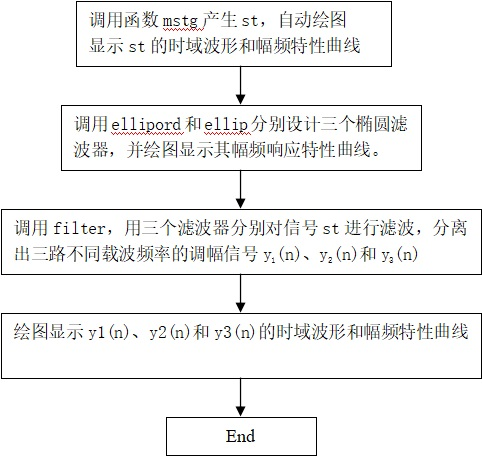
\includegraphics{mstg.jpg}
\caption{mstg}
\end{figure}

    \subsubsection{5.思考题}\label{ux601dux8003ux9898}

\begin{itemize}
\tightlist
\item
  (1)请阅读信号产生函数mstg,确定三路调幅信号的载波频率和调制信号频率。
\item
  (2)信号产生函数mstg中采样点数N=800,对st进行N点FFT可以得到6根理想谱线。如果取N=1000,可否得到6根理想谱线?为什么?N=2000呢?请改变函数mstg中采样点数N的值,观察频谱图验证您的判断是否正确。
\item
  (3)修改信号产生函数mstg,给每路调幅信号加入载波成分,产生调幅(AM)信号,重复本实验,观察AM信号与抑制载波调幅信号的时域波形及其频谱的差别。
\end{itemize}

提示:AM信号表示式:\[s(t)=[1+cos(2\pi f_0 t)]cos(2\pi f_c t)\]

答: - (1)在代码中已经做详细介绍 -
(2)其值必须是400的倍数,1800不是400的倍数,所以不行。而2000是400的倍数,所以可以。
-
(3)因为信号st是周期序列,谱分析时要求观察时间为整数倍周期。所以,本题的一般解答方法是,先确定信号st的周期,在判断所给采样点数N对应的观察时间Tp=NT是否为st的整数个周期。但信号产生函数mstg产生的信号st共有6个频率成分,求其周期比较麻烦,故采用下面的方法解答。:
-
分析发现,st的每个频率成分都是25Hz的整数倍。采样频率Fs=10kHz=25×400Hz,即在25Hz的正弦波的1个周期中采样400点。所以,当N为400的整数倍时一定为st的整数个周期。因此,采样点数N=800和N=2000时,对st进行N点FFT可以得到6根理想谱线。如果取N=1000,不是400的整数倍,不能得到6根理想谱线。

    \subsubsection{6.实验源码}\label{ux5b9eux9a8cux6e90ux7801}

    \begin{Verbatim}[commandchars=\\\{\}]
{\color{incolor}In [{\color{incolor}1}]:} \PY{k+kn}{import} \PY{n+nn}{numpy} \PY{k}{as} \PY{n+nn}{np}
        \PY{k+kn}{import} \PY{n+nn}{matplotlib}\PY{n+nn}{.}\PY{n+nn}{pyplot} \PY{k}{as} \PY{n+nn}{plt}
        \PY{k+kn}{import} \PY{n+nn}{seaborn} \PY{k}{as} \PY{n+nn}{sns}
        \PY{k+kn}{import} \PY{n+nn}{scipy}\PY{n+nn}{.}\PY{n+nn}{signal} \PY{k}{as} \PY{n+nn}{signal}
\end{Verbatim}


    \begin{Verbatim}[commandchars=\\\{\}]
{\color{incolor}In [{\color{incolor}2}]:} \PY{c+c1}{\PYZsh{}作图时中文显示}
        \PY{k+kn}{import} \PY{n+nn}{matplotlib}\PY{n+nn}{.}\PY{n+nn}{pyplot} \PY{k}{as} \PY{n+nn}{plt}
        \PY{n}{plt}\PY{o}{.}\PY{n}{rc}\PY{p}{(}\PY{l+s+s1}{\PYZsq{}}\PY{l+s+s1}{font}\PY{l+s+s1}{\PYZsq{}}\PY{p}{,} \PY{n}{family}\PY{o}{=}\PY{l+s+s1}{\PYZsq{}}\PY{l+s+s1}{SimHei}\PY{l+s+s1}{\PYZsq{}}\PY{p}{,} \PY{n}{size}\PY{o}{=}\PY{l+m+mi}{14}\PY{p}{)}
        \PY{n}{plt}\PY{o}{.}\PY{n}{rcParams}\PY{p}{[}\PY{l+s+s1}{\PYZsq{}}\PY{l+s+s1}{axes.unicode\PYZus{}minus}\PY{l+s+s1}{\PYZsq{}}\PY{p}{]} \PY{o}{=} \PY{k+kc}{False}
\end{Verbatim}


    \begin{Verbatim}[commandchars=\\\{\}]
{\color{incolor}In [{\color{incolor}3}]:} \PY{k}{def} \PY{n+nf}{mstg}\PY{p}{(}\PY{p}{)}\PY{p}{:}
            \PY{c+c1}{\PYZsh{}产生信号序列向量st,并显示st的时域波形和频谱}
            \PY{c+c1}{\PYZsh{}st=mstg 返回三路调幅信号相加形成的混合信号,长度N=1600}
            \PY{c+c1}{\PYZsh{}N为信号st的长度}
            \PY{n}{N}\PY{o}{=}\PY{l+m+mi}{800}
            \PY{c+c1}{\PYZsh{}采样频率Fs=10 kHz, Tp为采样时间}
            \PY{n}{Fs}\PY{o}{=}\PY{l+m+mi}{10000}
            \PY{n}{T}\PY{o}{=}\PY{l+m+mi}{1}\PY{o}{/}\PY{n}{Fs}
            \PY{n}{Tp}\PY{o}{=}\PY{n}{N}\PY{o}{*}\PY{n}{T}
            
            \PY{n}{t}\PY{o}{=}\PY{n}{np}\PY{o}{.}\PY{n}{arange}\PY{p}{(}\PY{l+m+mi}{0}\PY{p}{,}\PY{n}{N}\PY{o}{*}\PY{n}{T}\PY{p}{,}\PY{n}{T}\PY{p}{)}
            \PY{n}{k}\PY{o}{=}\PY{n}{np}\PY{o}{.}\PY{n}{arange}\PY{p}{(}\PY{l+m+mi}{0}\PY{p}{,}\PY{n}{N}\PY{p}{)}
            \PY{n}{f}\PY{o}{=}\PY{n}{k}\PY{o}{/}\PY{n}{Tp}
            
            \PY{c+c1}{\PYZsh{}第1路调幅信号的载波频率fc1=1000 Hz}
            \PY{n}{fc1}\PY{o}{=}\PY{n}{Fs}\PY{o}{/}\PY{l+m+mi}{10}
            \PY{c+c1}{\PYZsh{}第1路调幅信号的调制信号频率fm1=100 Hz}
            \PY{n}{fm1}\PY{o}{=}\PY{n}{fc1}\PY{o}{/}\PY{l+m+mi}{10}
            
            \PY{c+c1}{\PYZsh{}第2路调幅信号的载波频率fc2=500 Hz}
            \PY{n}{fc2}\PY{o}{=}\PY{n}{Fs}\PY{o}{/}\PY{l+m+mi}{20}
            \PY{c+c1}{\PYZsh{}第2路调幅信号的调制信号频率fm2=50 Hz}
            \PY{n}{fm2}\PY{o}{=}\PY{n}{fc2}\PY{o}{/}\PY{l+m+mi}{10}
            
            \PY{c+c1}{\PYZsh{}第3路调幅信号的载波频率fc3=250 Hz}
            \PY{n}{fc3}\PY{o}{=}\PY{n}{Fs}\PY{o}{/}\PY{l+m+mi}{40}
            \PY{c+c1}{\PYZsh{}第3路调幅信号的调制信号频率fm3=25 Hz}
            \PY{n}{fm3}\PY{o}{=}\PY{n}{fc3}\PY{o}{/}\PY{l+m+mi}{10}
            
            \PY{c+c1}{\PYZsh{}产生第1路调幅信号}
            \PY{n}{xt1}\PY{o}{=}\PY{n}{np}\PY{o}{.}\PY{n}{cos}\PY{p}{(}\PY{l+m+mi}{2}\PY{o}{*}\PY{n}{np}\PY{o}{.}\PY{n}{pi}\PY{o}{*}\PY{n}{fm1}\PY{o}{*}\PY{n}{t}\PY{p}{)}\PY{o}{*}\PY{n}{np}\PY{o}{.}\PY{n}{cos}\PY{p}{(}\PY{l+m+mi}{2}\PY{o}{*}\PY{n}{np}\PY{o}{.}\PY{n}{pi}\PY{o}{*}\PY{n}{fc1}\PY{o}{*}\PY{n}{t}\PY{p}{)}
            \PY{c+c1}{\PYZsh{}产生第2路调幅信号}
            \PY{n}{xt2}\PY{o}{=}\PY{n}{np}\PY{o}{.}\PY{n}{cos}\PY{p}{(}\PY{l+m+mi}{2}\PY{o}{*}\PY{n}{np}\PY{o}{.}\PY{n}{pi}\PY{o}{*}\PY{n}{fm2}\PY{o}{*}\PY{n}{t}\PY{p}{)}\PY{o}{*}\PY{n}{np}\PY{o}{.}\PY{n}{cos}\PY{p}{(}\PY{l+m+mi}{2}\PY{o}{*}\PY{n}{np}\PY{o}{.}\PY{n}{pi}\PY{o}{*}\PY{n}{fc2}\PY{o}{*}\PY{n}{t}\PY{p}{)}
            \PY{c+c1}{\PYZsh{}产生第3路调幅信号}
            \PY{n}{xt3}\PY{o}{=}\PY{n}{np}\PY{o}{.}\PY{n}{cos}\PY{p}{(}\PY{l+m+mi}{2}\PY{o}{*}\PY{n}{np}\PY{o}{.}\PY{n}{pi}\PY{o}{*}\PY{n}{fm3}\PY{o}{*}\PY{n}{t}\PY{p}{)}\PY{o}{*}\PY{n}{np}\PY{o}{.}\PY{n}{cos}\PY{p}{(}\PY{l+m+mi}{2}\PY{o}{*}\PY{n}{np}\PY{o}{.}\PY{n}{pi}\PY{o}{*}\PY{n}{fc3}\PY{o}{*}\PY{n}{t}\PY{p}{)}
            
            \PY{c+c1}{\PYZsh{}三路调幅信号相加}
            \PY{n}{st}\PY{o}{=}\PY{n}{xt1}\PY{o}{+}\PY{n}{xt2}\PY{o}{+}\PY{n}{xt3}
            \PY{c+c1}{\PYZsh{}计算信号st的频谱}
            \PY{n}{fxt}\PY{o}{=}\PY{n}{np}\PY{o}{.}\PY{n}{fft}\PY{o}{.}\PY{n}{fft}\PY{p}{(}\PY{n}{st}\PY{p}{,}\PY{n}{N}\PY{p}{)}
        
            \PY{c+c1}{\PYZsh{}以下为绘图部分,绘制st的时域波形和幅频特性曲线}
        
            \PY{l+s+sd}{\PYZsq{}\PYZsq{}\PYZsq{}    }
        \PY{l+s+sd}{    fig,axxr=plt.subplots(3,1,figsize=(14,16))}
        \PY{l+s+sd}{    axxr[0].plot(t,st)}
        \PY{l+s+sd}{    axxr[0].set\PYZus{}title(\PYZdq{}(a) s(t)的波形\PYZdq{})}
        \PY{l+s+sd}{    axxr[0].set\PYZus{}xlabel(\PYZdq{}t/s\PYZdq{})}
        \PY{l+s+sd}{    axxr[0].set\PYZus{}ylabel(\PYZdq{}s(t)\PYZdq{})}
        \PY{l+s+sd}{    axxr[1].stem(f,abs(fxt)/np.max(abs(fxt)),\PYZsq{}\PYZhy{}\PYZhy{}\PYZsq{})}
        \PY{l+s+sd}{    axxr[1].set\PYZus{}title(\PYZdq{}(b) s(t)的频谱\PYZdq{})}
        \PY{l+s+sd}{    axxr[1].set\PYZus{}xlabel(\PYZdq{}f/Hz\PYZdq{})}
        \PY{l+s+sd}{    axxr[1].set\PYZus{}ylabel(\PYZdq{}幅度\PYZdq{})}
        \PY{l+s+sd}{    \PYZsq{}\PYZsq{}\PYZsq{}}
        
            \PY{k}{return} \PY{n}{st}
\end{Verbatim}


    \begin{Verbatim}[commandchars=\\\{\}]
{\color{incolor}In [{\color{incolor}4}]:} \PY{k}{def} \PY{n+nf}{mstg1}\PY{p}{(}\PY{p}{)}\PY{p}{:}
            \PY{c+c1}{\PYZsh{}产生信号序列向量st,并显示st的时域波形和频谱}
            \PY{c+c1}{\PYZsh{}st=mstg 返回三路调幅信号相加形成的混合信号,长度N=1600}
            \PY{c+c1}{\PYZsh{}N为信号st的长度}
            \PY{n}{N}\PY{o}{=}\PY{l+m+mi}{800}
            \PY{c+c1}{\PYZsh{}采样频率Fs=10 kHz, Tp为采样时间}
            \PY{n}{Fs}\PY{o}{=}\PY{l+m+mi}{10000}
            \PY{n}{T}\PY{o}{=}\PY{l+m+mi}{1}\PY{o}{/}\PY{n}{Fs}
            \PY{n}{Tp}\PY{o}{=}\PY{n}{N}\PY{o}{*}\PY{n}{T}
            
            \PY{n}{t}\PY{o}{=}\PY{n}{np}\PY{o}{.}\PY{n}{arange}\PY{p}{(}\PY{l+m+mi}{0}\PY{p}{,}\PY{n}{N}\PY{o}{*}\PY{n}{T}\PY{p}{,}\PY{n}{T}\PY{p}{)}
            \PY{n}{k}\PY{o}{=}\PY{n}{np}\PY{o}{.}\PY{n}{arange}\PY{p}{(}\PY{l+m+mi}{0}\PY{p}{,}\PY{n}{N}\PY{p}{)}
            \PY{n}{f}\PY{o}{=}\PY{n}{k}\PY{o}{/}\PY{n}{Tp}
            
            \PY{c+c1}{\PYZsh{}第1路调幅信号的载波频率fc1=1000 Hz}
            \PY{n}{fc1}\PY{o}{=}\PY{n}{Fs}\PY{o}{/}\PY{l+m+mi}{10}
            \PY{c+c1}{\PYZsh{}第1路调幅信号的调制信号频率fm1=100 Hz}
            \PY{n}{fm1}\PY{o}{=}\PY{n}{fc1}\PY{o}{/}\PY{l+m+mi}{10}
            
            \PY{c+c1}{\PYZsh{}第2路调幅信号的载波频率fc2=500 Hz}
            \PY{n}{fc2}\PY{o}{=}\PY{n}{Fs}\PY{o}{/}\PY{l+m+mi}{20}
            \PY{c+c1}{\PYZsh{}第2路调幅信号的调制信号频率fm2=50 Hz}
            \PY{n}{fm2}\PY{o}{=}\PY{n}{fc2}\PY{o}{/}\PY{l+m+mi}{10}
            
            \PY{c+c1}{\PYZsh{}第3路调幅信号的载波频率fc3=250 Hz}
            \PY{n}{fc3}\PY{o}{=}\PY{n}{Fs}\PY{o}{/}\PY{l+m+mi}{40}
            \PY{c+c1}{\PYZsh{}第3路调幅信号的调制信号频率fm3=25 Hz}
            \PY{n}{fm3}\PY{o}{=}\PY{n}{fc3}\PY{o}{/}\PY{l+m+mi}{10}
            
            \PY{c+c1}{\PYZsh{}产生第1路调幅信号}
            \PY{n}{xt1}\PY{o}{=}\PY{n}{np}\PY{o}{.}\PY{n}{cos}\PY{p}{(}\PY{l+m+mi}{2}\PY{o}{*}\PY{n}{np}\PY{o}{.}\PY{n}{pi}\PY{o}{*}\PY{n}{fm1}\PY{o}{*}\PY{n}{t}\PY{p}{)}\PY{o}{*}\PY{n}{np}\PY{o}{.}\PY{n}{cos}\PY{p}{(}\PY{l+m+mi}{2}\PY{o}{*}\PY{n}{np}\PY{o}{.}\PY{n}{pi}\PY{o}{*}\PY{n}{fc1}\PY{o}{*}\PY{n}{t}\PY{p}{)}
            \PY{c+c1}{\PYZsh{}产生第2路调幅信号}
            \PY{n}{xt2}\PY{o}{=}\PY{n}{np}\PY{o}{.}\PY{n}{cos}\PY{p}{(}\PY{l+m+mi}{2}\PY{o}{*}\PY{n}{np}\PY{o}{.}\PY{n}{pi}\PY{o}{*}\PY{n}{fm2}\PY{o}{*}\PY{n}{t}\PY{p}{)}\PY{o}{*}\PY{n}{np}\PY{o}{.}\PY{n}{cos}\PY{p}{(}\PY{l+m+mi}{2}\PY{o}{*}\PY{n}{np}\PY{o}{.}\PY{n}{pi}\PY{o}{*}\PY{n}{fc2}\PY{o}{*}\PY{n}{t}\PY{p}{)}
            \PY{c+c1}{\PYZsh{}产生第3路调幅信号}
            \PY{n}{xt3}\PY{o}{=}\PY{n}{np}\PY{o}{.}\PY{n}{cos}\PY{p}{(}\PY{l+m+mi}{2}\PY{o}{*}\PY{n}{np}\PY{o}{.}\PY{n}{pi}\PY{o}{*}\PY{n}{fm3}\PY{o}{*}\PY{n}{t}\PY{p}{)}\PY{o}{*}\PY{n}{np}\PY{o}{.}\PY{n}{cos}\PY{p}{(}\PY{l+m+mi}{2}\PY{o}{*}\PY{n}{np}\PY{o}{.}\PY{n}{pi}\PY{o}{*}\PY{n}{fc3}\PY{o}{*}\PY{n}{t}\PY{p}{)}
        
            \PY{c+c1}{\PYZsh{}三路调幅信号相加}
            \PY{n}{st}\PY{o}{=}\PY{n}{xt1}\PY{o}{+}\PY{n}{xt2}\PY{o}{+}\PY{n}{xt3}
            \PY{c+c1}{\PYZsh{}计算信号st的频谱}
            \PY{n}{fxt}\PY{o}{=}\PY{n}{np}\PY{o}{.}\PY{n}{fft}\PY{o}{.}\PY{n}{fft}\PY{p}{(}\PY{n}{st}\PY{p}{,}\PY{n}{N}\PY{p}{)}
        
            \PY{c+c1}{\PYZsh{}以下为绘图部分,绘制st的时域波形和幅频特性曲线}
           
            \PY{n}{fig}\PY{p}{,}\PY{n}{axxr}\PY{o}{=}\PY{n}{plt}\PY{o}{.}\PY{n}{subplots}\PY{p}{(}\PY{l+m+mi}{2}\PY{p}{,}\PY{l+m+mi}{1}\PY{p}{,}\PY{n}{figsize}\PY{o}{=}\PY{p}{(}\PY{l+m+mi}{14}\PY{p}{,}\PY{l+m+mi}{16}\PY{p}{)}\PY{p}{)}
            \PY{n}{axxr}\PY{p}{[}\PY{l+m+mi}{0}\PY{p}{]}\PY{o}{.}\PY{n}{plot}\PY{p}{(}\PY{n}{t}\PY{p}{,}\PY{n}{st}\PY{p}{)}
            \PY{n}{axxr}\PY{p}{[}\PY{l+m+mi}{0}\PY{p}{]}\PY{o}{.}\PY{n}{set\PYZus{}title}\PY{p}{(}\PY{l+s+s2}{\PYZdq{}}\PY{l+s+s2}{(a) s(t)的波形}\PY{l+s+s2}{\PYZdq{}}\PY{p}{)}
            \PY{n}{axxr}\PY{p}{[}\PY{l+m+mi}{0}\PY{p}{]}\PY{o}{.}\PY{n}{set\PYZus{}xlabel}\PY{p}{(}\PY{l+s+s2}{\PYZdq{}}\PY{l+s+s2}{t/s}\PY{l+s+s2}{\PYZdq{}}\PY{p}{)}
            \PY{n}{axxr}\PY{p}{[}\PY{l+m+mi}{0}\PY{p}{]}\PY{o}{.}\PY{n}{set\PYZus{}ylabel}\PY{p}{(}\PY{l+s+s2}{\PYZdq{}}\PY{l+s+s2}{s(t)}\PY{l+s+s2}{\PYZdq{}}\PY{p}{)}
            \PY{n}{axxr}\PY{p}{[}\PY{l+m+mi}{1}\PY{p}{]}\PY{o}{.}\PY{n}{stem}\PY{p}{(}\PY{n}{f}\PY{p}{,}\PY{n+nb}{abs}\PY{p}{(}\PY{n}{fxt}\PY{p}{)}\PY{o}{/}\PY{n}{np}\PY{o}{.}\PY{n}{max}\PY{p}{(}\PY{n+nb}{abs}\PY{p}{(}\PY{n}{fxt}\PY{p}{)}\PY{p}{)}\PY{p}{,}\PY{l+s+s1}{\PYZsq{}}\PY{l+s+s1}{\PYZhy{}\PYZhy{}}\PY{l+s+s1}{\PYZsq{}}\PY{p}{)}
            \PY{n}{axxr}\PY{p}{[}\PY{l+m+mi}{1}\PY{p}{]}\PY{o}{.}\PY{n}{set\PYZus{}title}\PY{p}{(}\PY{l+s+s2}{\PYZdq{}}\PY{l+s+s2}{(b) s(t)的频谱}\PY{l+s+s2}{\PYZdq{}}\PY{p}{)}
            \PY{n}{axxr}\PY{p}{[}\PY{l+m+mi}{1}\PY{p}{]}\PY{o}{.}\PY{n}{set\PYZus{}xlim}\PY{p}{(}\PY{n}{xmax}\PY{o}{=}\PY{l+m+mi}{2000}\PY{p}{)}
            \PY{n}{axxr}\PY{p}{[}\PY{l+m+mi}{1}\PY{p}{]}\PY{o}{.}\PY{n}{set\PYZus{}xlabel}\PY{p}{(}\PY{l+s+s2}{\PYZdq{}}\PY{l+s+s2}{f/Hz}\PY{l+s+s2}{\PYZdq{}}\PY{p}{)}
            \PY{n}{axxr}\PY{p}{[}\PY{l+m+mi}{1}\PY{p}{]}\PY{o}{.}\PY{n}{set\PYZus{}ylabel}\PY{p}{(}\PY{l+s+s2}{\PYZdq{}}\PY{l+s+s2}{幅度}\PY{l+s+s2}{\PYZdq{}}\PY{p}{)}
            
            \PY{c+c1}{\PYZsh{}return st}
        \PY{n}{mstg1}\PY{p}{(}\PY{p}{)}
\end{Verbatim}


    \begin{center}
    \adjustimage{max size={0.9\linewidth}{0.9\paperheight}}{output_6_0.png}
    \end{center}
    { \hspace*{\fill} \\}
    
    \begin{Verbatim}[commandchars=\\\{\}]
{\color{incolor}In [{\color{incolor}5}]:} \PY{c+c1}{\PYZsh{}时域离散系统损耗函数绘图}
        \PY{k}{def} \PY{n+nf}{myplot}\PY{p}{(}\PY{n}{B}\PY{p}{,}\PY{n}{A}\PY{p}{)}\PY{p}{:}
            \PY{c+c1}{\PYZsh{}B为系统函数分子多项式系数向量}
            \PY{c+c1}{\PYZsh{}A为系统函数分母多项式系数向量}
            \PY{c+c1}{\PYZsh{}计算数字滤波器的频率响应}
            \PY{p}{[}\PY{n}{W}\PY{p}{,}\PY{n}{H}\PY{p}{]}\PY{o}{=}\PY{n}{signal}\PY{o}{.}\PY{n}{freqz}\PY{p}{(}\PY{n}{B}\PY{p}{,}\PY{n}{A}\PY{p}{,}\PY{l+m+mi}{1000}\PY{p}{)}        \PY{c+c1}{\PYZsh{}数字滤波器的频率响应}
            \PY{n}{plt}\PY{o}{.}\PY{n}{plot}\PY{p}{(}\PY{n}{W}\PY{p}{,}\PY{l+m+mi}{20}\PY{o}{*}\PY{n}{np}\PY{o}{.}\PY{n}{log10}\PY{p}{(}\PY{n+nb}{abs}\PY{p}{(}\PY{n}{H}\PY{p}{)}\PY{p}{)}\PY{p}{)}
            \PY{n}{plt}\PY{o}{.}\PY{n}{grid}\PY{p}{(}\PY{k+kc}{True}\PY{p}{)}
            \PY{n}{plt}\PY{o}{.}\PY{n}{xlabel}\PY{p}{(}\PY{l+s+s2}{\PYZdq{}}\PY{l+s+s2}{\PYZbs{}}\PY{l+s+s2}{omega/}\PY{l+s+s2}{\PYZbs{}}\PY{l+s+s2}{pi}\PY{l+s+s2}{\PYZdq{}}\PY{p}{)}
            \PY{n}{plt}\PY{o}{.}\PY{n}{ylabel}\PY{p}{(}\PY{l+s+s1}{\PYZsq{}}\PY{l+s+s1}{幅度(dB)}\PY{l+s+s1}{\PYZsq{}}\PY{p}{)}
            \PY{n}{plt}\PY{o}{.}\PY{n}{title}\PY{p}{(}\PY{l+s+s1}{\PYZsq{}}\PY{l+s+s1}{损耗函数曲线}\PY{l+s+s1}{\PYZsq{}}\PY{p}{)}
\end{Verbatim}


    \begin{Verbatim}[commandchars=\\\{\}]
{\color{incolor}In [{\color{incolor}6}]:} \PY{c+c1}{\PYZsh{}时域序列连续曲线绘图函数}
        \PY{k}{def} \PY{n+nf}{tplot}\PY{p}{(}\PY{n}{xn}\PY{p}{,}\PY{n}{T}\PY{p}{,}\PY{n}{yn}\PY{p}{)}\PY{p}{:}
            \PY{c+c1}{\PYZsh{}xn:信号数据序列,yn:绘图信号的纵坐标名字(字符串)}
            \PY{c+c1}{\PYZsh{}T为采样间隔}
            \PY{n}{n}\PY{o}{=}\PY{n}{np}\PY{o}{.}\PY{n}{arange}\PY{p}{(}\PY{n+nb}{len}\PY{p}{(}\PY{n}{xn}\PY{p}{)}\PY{p}{)}
            \PY{n}{t}\PY{o}{=}\PY{n}{n}\PY{o}{*}\PY{n}{T}
            \PY{n}{plt}\PY{o}{.}\PY{n}{plot}\PY{p}{(}\PY{n}{t}\PY{p}{,}\PY{n}{xn}\PY{p}{)}
            \PY{n}{plt}\PY{o}{.}\PY{n}{xlabel}\PY{p}{(}\PY{l+s+s2}{\PYZdq{}}\PY{l+s+s2}{t/s}\PY{l+s+s2}{\PYZdq{}}\PY{p}{)}
            \PY{n}{plt}\PY{o}{.}\PY{n}{ylabel}\PY{p}{(}\PY{n}{yn}\PY{p}{)}
            \PY{n}{plt}\PY{o}{.}\PY{n}{title}\PY{p}{(}\PY{l+s+s2}{\PYZdq{}}\PY{l+s+s2}{滤波后的时域波形}\PY{l+s+s2}{\PYZdq{}}\PY{p}{)}
\end{Verbatim}


    \begin{Verbatim}[commandchars=\\\{\}]
{\color{incolor}In [{\color{incolor}7}]:} \PY{c+c1}{\PYZsh{}IIR数字滤波器设计及软件实现}
        \PY{c+c1}{\PYZsh{}采样频率}
        \PY{n}{Fs}\PY{o}{=}\PY{l+m+mi}{10000}
        \PY{n}{T}\PY{o}{=}\PY{l+m+mi}{1}\PY{o}{/}\PY{n}{Fs}
        \PY{c+c1}{\PYZsh{}调用信号产生函数mstg产生由三路抑制载波调幅信号相加构成的复合信号st }
        \PY{n}{st}\PY{o}{=}\PY{n}{mstg}\PY{p}{(}\PY{p}{)}
\end{Verbatim}


    \begin{Verbatim}[commandchars=\\\{\}]
{\color{incolor}In [{\color{incolor}8}]:} \PY{c+c1}{\PYZsh{}低通滤波器设计与实现=========================}
        \PY{c+c1}{\PYZsh{}DF指标(低通滤波器的通、 阻带边界频率)}
        \PY{n}{fp}\PY{o}{=}\PY{l+m+mi}{280}
        \PY{n}{fs}\PY{o}{=}\PY{l+m+mi}{450}\PY{p}{;}
        \PY{n}{wp}\PY{o}{=}\PY{l+m+mi}{2}\PY{o}{*}\PY{n}{fp}\PY{o}{/}\PY{n}{Fs}
        \PY{n}{ws}\PY{o}{=}\PY{l+m+mi}{2}\PY{o}{*}\PY{n}{fs}\PY{o}{/}\PY{n}{Fs}
        \PY{n}{rp}\PY{o}{=}\PY{l+m+mf}{0.1}
        \PY{n}{rs}\PY{o}{=}\PY{l+m+mi}{60}\PY{p}{;}    
        \PY{c+c1}{\PYZsh{}调用ellipord计算椭圆DF阶数N和通带截止频率wp}
        \PY{p}{[}\PY{n}{N}\PY{p}{,}\PY{n}{wp}\PY{p}{]}\PY{o}{=}\PY{n}{signal}\PY{o}{.}\PY{n}{ellipord}\PY{p}{(}\PY{n}{wp}\PY{p}{,}\PY{n}{ws}\PY{p}{,}\PY{n}{rp}\PY{p}{,}\PY{n}{rs}\PY{p}{)}\PY{p}{;}      
        \PY{c+c1}{\PYZsh{}调用ellip计算椭圆带通DF系统函数系数向量B和A}
        \PY{p}{[}\PY{n}{B}\PY{p}{,}\PY{n}{A}\PY{p}{]}\PY{o}{=}\PY{n}{signal}\PY{o}{.}\PY{n}{ellip}\PY{p}{(}\PY{n}{N}\PY{p}{,}\PY{n}{rp}\PY{p}{,}\PY{n}{rs}\PY{p}{,}\PY{n}{wp}\PY{p}{)}\PY{p}{;}  
        \PY{c+c1}{\PYZsh{}低通滤波器设计与实现绘图部分}
        \PY{c+c1}{\PYZsh{}调用绘图函数myplot绘制损耗函数曲线}
        \PY{n}{plt}\PY{o}{.}\PY{n}{subplot}\PY{p}{(}\PY{l+m+mi}{2}\PY{p}{,}\PY{l+m+mi}{1}\PY{p}{,}\PY{l+m+mi}{1}\PY{p}{)}\PY{p}{;}
        \PY{n}{myplot}\PY{p}{(}\PY{n}{B}\PY{p}{,}\PY{n}{A}\PY{p}{)}\PY{p}{;}
        \PY{c+c1}{\PYZsh{}滤波器软件实现}
        \PY{n}{y1t}\PY{o}{=}\PY{n}{signal}\PY{o}{.}\PY{n}{lfilter}\PY{p}{(}\PY{n}{B}\PY{p}{,}\PY{n}{A}\PY{p}{,}\PY{n}{st}\PY{p}{)}\PY{p}{;}    
        \PY{c+c1}{\PYZsh{}调用绘图函数tplot绘制滤波器输出波形}
        \PY{n}{yt}\PY{o}{=}\PY{l+s+sa}{r}\PY{l+s+s1}{\PYZsq{}}\PY{l+s+s1}{y\PYZus{}1(t)\PYZdl{}}\PY{l+s+s1}{\PYZsq{}}\PY{p}{;}
        \PY{n}{plt}\PY{o}{.}\PY{n}{subplot}\PY{p}{(}\PY{l+m+mi}{2}\PY{p}{,}\PY{l+m+mi}{1}\PY{p}{,}\PY{l+m+mi}{2}\PY{p}{)}\PY{p}{;}
        \PY{n}{tplot}\PY{p}{(}\PY{n}{y1t}\PY{p}{,}\PY{n}{T}\PY{p}{,}\PY{n}{yt}\PY{p}{)}\PY{p}{;}  
\end{Verbatim}


    \begin{center}
    \adjustimage{max size={0.9\linewidth}{0.9\paperheight}}{output_10_0.png}
    \end{center}
    { \hspace*{\fill} \\}
    
    \begin{Verbatim}[commandchars=\\\{\}]
{\color{incolor}In [{\color{incolor}9}]:} \PY{c+c1}{\PYZsh{}带通滤波器设计与实现=========================}
        \PY{n}{fpl}\PY{o}{=}\PY{l+m+mi}{440}\PY{p}{;}
        \PY{n}{fpu}\PY{o}{=}\PY{l+m+mi}{560}\PY{p}{;}
        \PY{n}{fsl}\PY{o}{=}\PY{l+m+mi}{275}\PY{p}{;}
        \PY{n}{fsu}\PY{o}{=}\PY{l+m+mi}{900}\PY{p}{;}
        \PY{n}{wp}\PY{o}{=}\PY{p}{[}\PY{l+m+mi}{2}\PY{o}{*}\PY{n}{fpl}\PY{o}{/}\PY{n}{Fs}\PY{p}{,}\PY{l+m+mi}{2}\PY{o}{*}\PY{n}{fpu}\PY{o}{/}\PY{n}{Fs}\PY{p}{]}\PY{p}{;} 
        \PY{n}{ws}\PY{o}{=}\PY{p}{[}\PY{l+m+mi}{2}\PY{o}{*}\PY{n}{fsl}\PY{o}{/}\PY{n}{Fs}\PY{p}{,}\PY{l+m+mi}{2}\PY{o}{*}\PY{n}{fsu}\PY{o}{/}\PY{n}{Fs}\PY{p}{]}\PY{p}{;}
        \PY{n}{rp}\PY{o}{=}\PY{l+m+mf}{0.1}\PY{p}{;}
        \PY{n}{rs}\PY{o}{=}\PY{l+m+mi}{60}\PY{p}{;} 
        \PY{c+c1}{\PYZsh{}调用ellipord计算椭圆DF阶数N和通带截止频率wp}
        \PY{p}{[}\PY{n}{N}\PY{p}{,}\PY{n}{wp}\PY{p}{]}\PY{o}{=}\PY{n}{signal}\PY{o}{.}\PY{n}{ellipord}\PY{p}{(}\PY{n}{wp}\PY{p}{,}\PY{n}{ws}\PY{p}{,}\PY{n}{rp}\PY{p}{,}\PY{n}{rs}\PY{p}{)}\PY{p}{;}
        \PY{c+c1}{\PYZsh{}调用ellip计算椭圆带通DF系统函数系数向量B和A}
        \PY{c+c1}{\PYZsh{}[B,A]=signal.ellip(N,rp,rs,wp); }
        \PY{p}{[}\PY{n}{B}\PY{p}{,}\PY{n}{A}\PY{p}{]}\PY{o}{=}\PY{n}{signal}\PY{o}{.}\PY{n}{ellip}\PY{p}{(}\PY{n}{N}\PY{p}{,}\PY{n}{rp}\PY{p}{,}\PY{n}{rs}\PY{p}{,}\PY{n}{wp}\PY{p}{,}\PY{l+s+s1}{\PYZsq{}}\PY{l+s+s1}{bandpass}\PY{l+s+s1}{\PYZsq{}}\PY{p}{)}\PY{p}{;}
        \PY{c+c1}{\PYZsh{}滤波器软件实现}
        \PY{n}{y2t}\PY{o}{=}\PY{n}{signal}\PY{o}{.}\PY{n}{lfilter}\PY{p}{(}\PY{n}{B}\PY{p}{,}\PY{n}{A}\PY{p}{,}\PY{n}{st}\PY{p}{)}\PY{p}{;}     
\end{Verbatim}


    \begin{Verbatim}[commandchars=\\\{\}]
{\color{incolor}In [{\color{incolor}10}]:} \PY{c+c1}{\PYZsh{}带通滤波器设计与实现绘图部分}
         \PY{c+c1}{\PYZsh{}调用绘图函数myplot绘制损耗函数曲线}
         \PY{n}{plt}\PY{o}{.}\PY{n}{subplot}\PY{p}{(}\PY{l+m+mi}{2}\PY{p}{,}\PY{l+m+mi}{1}\PY{p}{,}\PY{l+m+mi}{1}\PY{p}{)}\PY{p}{;}
         \PY{n}{myplot}\PY{p}{(}\PY{n}{B}\PY{p}{,}\PY{n}{A}\PY{p}{)}\PY{p}{;}
         \PY{c+c1}{\PYZsh{}调用绘图函数tplot绘制滤波器输出波形}
         \PY{n}{yt}\PY{o}{=}\PY{l+s+sa}{r}\PY{l+s+s1}{\PYZsq{}}\PY{l+s+s1}{\PYZdl{}y\PYZus{}2(t)\PYZdl{}}\PY{l+s+s1}{\PYZsq{}}\PY{p}{;}
         \PY{n}{plt}\PY{o}{.}\PY{n}{subplot}\PY{p}{(}\PY{l+m+mi}{2}\PY{p}{,}\PY{l+m+mi}{1}\PY{p}{,}\PY{l+m+mi}{2}\PY{p}{)}\PY{p}{;}
         \PY{n}{tplot}\PY{p}{(}\PY{n}{y2t}\PY{p}{,}\PY{n}{T}\PY{p}{,}\PY{n}{yt}\PY{p}{)}\PY{p}{;}      
\end{Verbatim}


    \begin{center}
    \adjustimage{max size={0.9\linewidth}{0.9\paperheight}}{output_12_0.png}
    \end{center}
    { \hspace*{\fill} \\}
    
    \begin{Verbatim}[commandchars=\\\{\}]
{\color{incolor}In [{\color{incolor}11}]:} \PY{c+c1}{\PYZsh{}高通滤波器设计与实现===========================}
         \PY{n}{fp}\PY{o}{=}\PY{l+m+mi}{890}\PY{p}{;}
         \PY{n}{fs}\PY{o}{=}\PY{l+m+mi}{600}\PY{p}{;}
         \PY{n}{wp}\PY{o}{=}\PY{l+m+mi}{2}\PY{o}{*}\PY{n}{fp}\PY{o}{/}\PY{n}{Fs}\PY{p}{;} 
         \PY{n}{ws}\PY{o}{=}\PY{l+m+mi}{2}\PY{o}{*}\PY{n}{fs}\PY{o}{/}\PY{n}{Fs}\PY{p}{;}
         \PY{n}{rp}\PY{o}{=}\PY{l+m+mf}{0.1}\PY{p}{;}
         \PY{n}{rs}\PY{o}{=}\PY{l+m+mi}{60}\PY{p}{;}    
         \PY{c+c1}{\PYZsh{}DF指标(低通滤波器的通、 阻带边界频率)}
         \PY{c+c1}{\PYZsh{}调用ellipord计算椭圆DF阶数N和通带\PYZpc{}截止频率wp}
         \PY{p}{[}\PY{n}{N}\PY{p}{,}\PY{n}{wp}\PY{p}{]}\PY{o}{=}\PY{n}{signal}\PY{o}{.}\PY{n}{ellipord}\PY{p}{(}\PY{n}{wp}\PY{p}{,}\PY{n}{ws}\PY{p}{,}\PY{n}{rp}\PY{p}{,}\PY{n}{rs}\PY{p}{)}\PY{p}{;}     
         \PY{c+c1}{\PYZsh{}调用ellip计算椭圆带通DF系统函数系数向量B和A}
         \PY{p}{[}\PY{n}{B}\PY{p}{,}\PY{n}{A}\PY{p}{]}\PY{o}{=}\PY{n}{signal}\PY{o}{.}\PY{n}{ellip}\PY{p}{(}\PY{n}{N}\PY{p}{,}\PY{n}{rp}\PY{p}{,}\PY{n}{rs}\PY{p}{,}\PY{n}{wp}\PY{p}{,}\PY{l+s+s1}{\PYZsq{}}\PY{l+s+s1}{high}\PY{l+s+s1}{\PYZsq{}}\PY{p}{)}\PY{p}{;}  
         \PY{c+c1}{\PYZsh{}滤波器软件实现}
         \PY{n}{y3t}\PY{o}{=}\PY{n}{signal}\PY{o}{.}\PY{n}{lfilter}\PY{p}{(}\PY{n}{B}\PY{p}{,}\PY{n}{A}\PY{p}{,}\PY{n}{st}\PY{p}{)}\PY{p}{;} 
\end{Verbatim}


    \begin{Verbatim}[commandchars=\\\{\}]
{\color{incolor}In [{\color{incolor}12}]:} \PY{c+c1}{\PYZsh{}高低通滤波器设计与实现绘图部分}
         \PY{c+c1}{\PYZsh{}调用绘图函数myplot绘制损耗函数曲线}
         \PY{n}{plt}\PY{o}{.}\PY{n}{subplot}\PY{p}{(}\PY{l+m+mi}{2}\PY{p}{,}\PY{l+m+mi}{1}\PY{p}{,}\PY{l+m+mi}{1}\PY{p}{)}\PY{p}{;}
         \PY{n}{myplot}\PY{p}{(}\PY{n}{B}\PY{p}{,}\PY{n}{A}\PY{p}{)}\PY{p}{;}
         \PY{c+c1}{\PYZsh{}调用绘图函数tplot绘制滤波器输出波形}
         \PY{n}{yt}\PY{o}{=}\PY{l+s+sa}{r}\PY{l+s+s1}{\PYZsq{}}\PY{l+s+s1}{\PYZdl{}y\PYZus{}3(t)\PYZdl{}}\PY{l+s+s1}{\PYZsq{}}\PY{p}{;}
         \PY{n}{plt}\PY{o}{.}\PY{n}{subplot}\PY{p}{(}\PY{l+m+mi}{2}\PY{p}{,}\PY{l+m+mi}{1}\PY{p}{,}\PY{l+m+mi}{2}\PY{p}{)}\PY{p}{;}
         \PY{n}{tplot}\PY{p}{(}\PY{n}{y3t}\PY{p}{,}\PY{n}{T}\PY{p}{,}\PY{n}{yt}\PY{p}{)}\PY{p}{;}    
\end{Verbatim}


    \begin{center}
    \adjustimage{max size={0.9\linewidth}{0.9\paperheight}}{output_14_0.png}
    \end{center}
    { \hspace*{\fill} \\}
    

    % Add a bibliography block to the postdoc
    
    
    
    \end{document}
